\section{Introduction}
Before a customer buys any product, the decision of whether or not he will buy it depends largely on his prior opinions about that product.
These opinions, in turn, have been built based on his opinions on relating companies or products and other customers' opinions about that product.
After having been experiencing the product, his posterior opinions on the product not only tell us about which features he likes or not.
His opinion also informs the retailer about the reasons why he bought the product, his expectations, needs and even more his personal information.
In a circle, his opinions will also affect the opinion of new customers and even the design of future products.
As a result, customers' opinions are the controllers behind every companies' good decisions.
They shape companies' marketing strategies, policies, and designs of products.
They judge which company is more competent than another.

\paragraph{Convolution Neural Networks and Recusive Neural Networks}
Convolution Neural Networks (CNNs) have been proven to be effective models for the task of sentence-level sentiment analysis~\cite{KimCNN}.
Although being a simple Convolution Neural Network architect on top of pre-trained word embedding channels, CNN-multichannel~\cite{KimCNN} was able to archive state-of-the-art performance\footnote{2014} on Stanford Sentiment Treebank with binary setting.
Despite its success, for dealing with the problem composing fixed size presentation vectors given variable-length input sentences, CNN-multichannel utilized max-over-time pooling layer~\cite{nlp-scratch}.
\textbf{Although max-over-time pooling largely simplified the network (which is good for preventing over-fit), this solution have a clear drawback: the vector presentation of a sentence only tell if a feature appears in the sentence or not, the information about position of the feature is ignored}.
The structure of CNN-multichannel is demonstrated in Fig.\ref{fig:CNN-multichannel}~\cite{KimCNN}.

\begin{figure*}[]
	\centering
	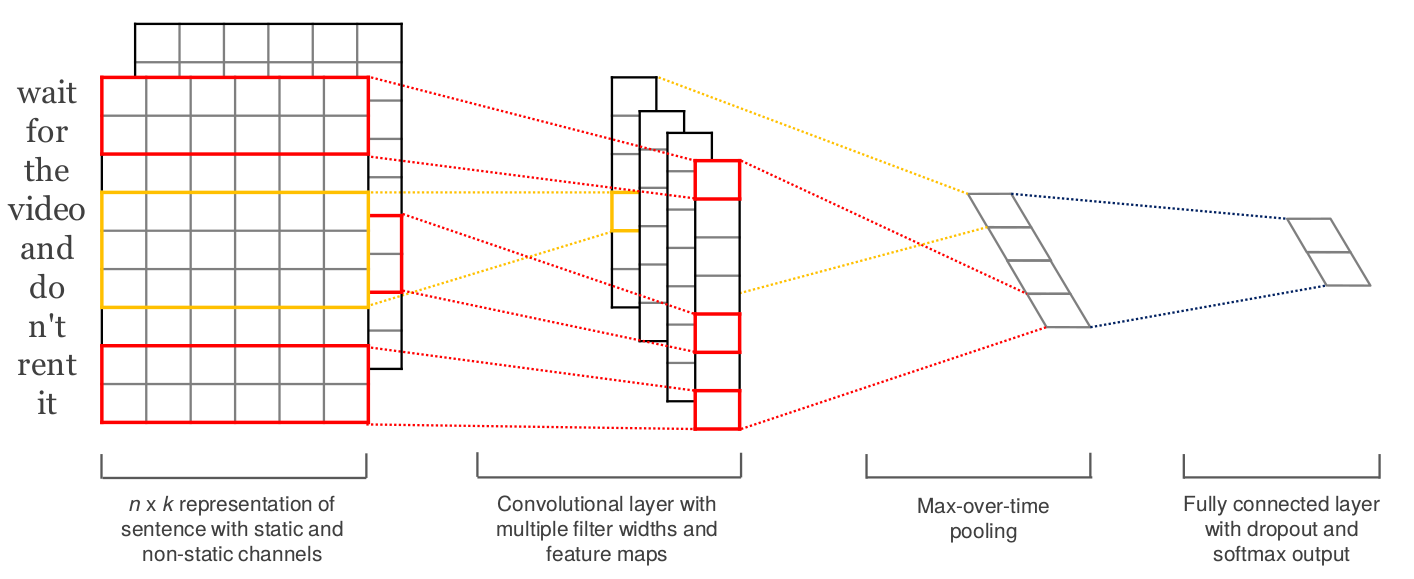
\includegraphics[scale=0.36]{figure/sentencecnn}
	\caption[CNN-multichannel]{Structure of CNN-multichannel. 
		At the convolution layer, each filter produces a feature map of the input sentence. 
		In turn, each feature map through the max-over-time pooling layer produces a feature in the vector presentation of the sentence}
	\label{fig:CNN-multichannel}
\end{figure*}

For dealing with the problem composing fixed size presentation vectors given variable-length input sentences, one intuitive solutions would be to apply Recurrent Neural Networks~\cite{cnn-rnn}.
Another more complicated solution is utilizing Recursive Neural Networks.
\textbf{Recursive Neural Networks have several advantages over Recurrent Neural Networks}~\cite{need-tree}~\cite{bowman-treevslstm}: 
\begin{itemize}
	\item In case the input sequence belongs to recursively defined language, given only a small subset of the data with limited length sentences, tree structures model have better ability to generalize compare to sequential ones.
	But when we increase the limited length sentences, the advantage of tree over sequential models decrease fast~\cite{bowman-treevslstm}. 
	\item Tree can breaks down complicated sentences into simpler phrases, which make it easier for generalization~\cite{knowledge-matter}~\cite{need-tree}.
	\item Some features which are far apart when a sentence is presented as sequence become closer when it is presented as tree~\cite{need-tree}.
\end{itemize}

\textbf{Tree-LSTMs also have some drawbacks}, these drawbacks including:
\begin{itemize}
	\item Sentences can be wrongly parsed, especially when comments are expressed in informal language.
	The performance of the system depends on the parser being used.
	\item At their leaf-module, Tree-LSTMs have only a simple logistic regression layer on top of the vector presentation of a single word at that position. 
\end{itemize}
\section{Related Work}
In recent years, the advancements of deep learning have led to dramatic improvements in the field of Sentiment Analysis:
\begin{description}
	\item [2013] Based on the theory that learning appropriate intermediate representations can lead to better generalisation~\cite{knowledge-matter}~\cite{tran-auto-encoder}, Socher and the co-authors augmented Rotten Tomatoes Movie Review  (RT-MR) dataset~\cite{Rotten-Tomato} with phrase-level sentiment labels (the new dataset was named Stanford Sentiment Treebank), in this way, any network can learn to correctly classify phrase-level sentiment, before it learns to classify sentence-level sentiment~\cite{socher2013recursive}. Along with the dataset, the authors also introduced three Recursive Neural Network, which inspired by the recursive structure of language ~\cite{socher2013recursive}.
	They were able to archive state of the art performance on SST test set (which is similar to RT-MR test set).
	Since then, this dataset has become the most popular dataset for the task of sentence-level sentiment analysis.
	
	In the same year, two other studies which have a large impact on the whole NLP community appeared.
	Mikolov and his partners introduced word2vec which has the ability to learn a certain level of syntactic and semantic relationships among words~\cite{word2vec}.
	Pre-learned word presentations have been used widely and become the “secret sauce” for the success of recent NLP systems~\cite{Luong_betterword}.
	
	Another research~\cite{GravesLSTM} popularized Long Short Term Memory Network (LSTM) and its "staked" variations (e.g. multilayer LSTM , Bidirectional LSTM).
	By mitigating the problem of gradient vanishing of RNNs, LSTMs and its variations become so popular that, we can find them in most NLP publications from 2014 to 2017.
	LSTMs is one of the first successful variation of RNNs which leads the way to many other more advanced RNNs variation~\cite{olah2016attention}.
	
	\item [2014] Applying only one layer CNN on multi-channel word embeddings, Yoon Kim successfully archived state of the art performance on SST (binary setting) as well as other datasets of different tasks~\cite{KimCNN}.
	This success attracted many future researches applying CNN on sentiment analysis~\cite{2-layer-cnn}~\cite{cnn-rnn}.
	
	Another research which we applied in our thesis is Glove method for training word embeddings~\cite{glove}.
	Different from word2vec, Glove vectors captures word co-occurrences globally in the corpus, whereas word2vec only captures local word co-occurrences in each window of its training examples~\cite{glove}.
	
	\item [2015] Combining recursive structure of Recursive Neural Networks~\cite{socher2013recursive} and LSTM~\cite{originLSTM}, Kai Sheng Tai, Socher and Christopher Manning introduced tree-structured LSTM  (TreeLSTM)~\cite{treeLSTM}.
	Their models archived state of the art performance on SST (fine-grained setting) and task of semantic relatedness (SemEval~2014, Task~1~\cite{SemeEvalTask1}).
	This success lead to multiple researches~\cite{need-tree}~\cite{bowman-treevslstm}~\cite{Graves_Nature2016} which aim to comparing tree-structured and sequential LSTM.
	The question is whether tree-structured networks are necessary or at least have some advantages over sequential architects when processing recursive-structured languages~\cite{need-tree}~\cite{bowman-treevslstm}.
	
	In the same year, there are two researches~\cite{ParagraphVec}~\cite{semisup-seq2seq} of Quoc V. Le which introduced several methods for unsupervised pre-training neural network models for NLP tasks.
	These methods help network models to mitigate over-fitting (which lead to better generalization) by allowing them to be pre-trained on large unlabeled datasets.
	We will apply several unsupervised pre-train methods in this thesis.
	
	\item [2016] Xingyou Wang and his partners combined convolutional and recurrent neural networks to archive staggering improvement on SST (both binary and fine-grained setting).
	Until now\footnote{July, 2017}, their models are state of the art on SST and also RT-MR~\cite{cnn-rnn}.
\end{description}


\section{Model Description}
\subsection{Word Embeddings and Matrix Representations of Phrases}
Embedding layer is a lookup table that converts input data (such as text) into its vector representation. Word embedding layer parameters are its embedding matrix $M  \in \mathbb{R}^{n \times d}$, where $n$ and $d$ are vocabulary size and embedding vector dimension, respectively. In practical, an embedding layer also comes with a vocabulary-index lookup table, which maps words with indexes, which has vector representation corresponding to the row in word embedding matrix.

The following steps are required once for each experiment:
\begin{itemize}
	\item Build vocabulary-index lookup table
	\item Init/Load word embedding matrix corresponding to vocabulary-index table
	\item Convert every sentence in dataset into indices using vocabulary-index table
\end{itemize}
Usually, indices are kept as dataset. Raw dataset (such as readable words) are discarded to free up memory. For each mini-batch, we use indices to look up word representation vector from embedding matrix. Embedding matrix represents of each sentence in dataset are not saved and needed look-up every mini-batch for the following reason.
\begin{itemize}
	\item Saved embedding matrix for each data sentences cost more memory than saving only indices and look-up in embedding layer.
	\item Embedding matrix contains trainable parameters and being updated every iteration.
\end{itemize}

Fig.\ref{fig:embeddinglayer} illustrates embedding layer component and describes the process of convert raw data sentence into its word representation.

\begin{figure}[H]
	\centering
	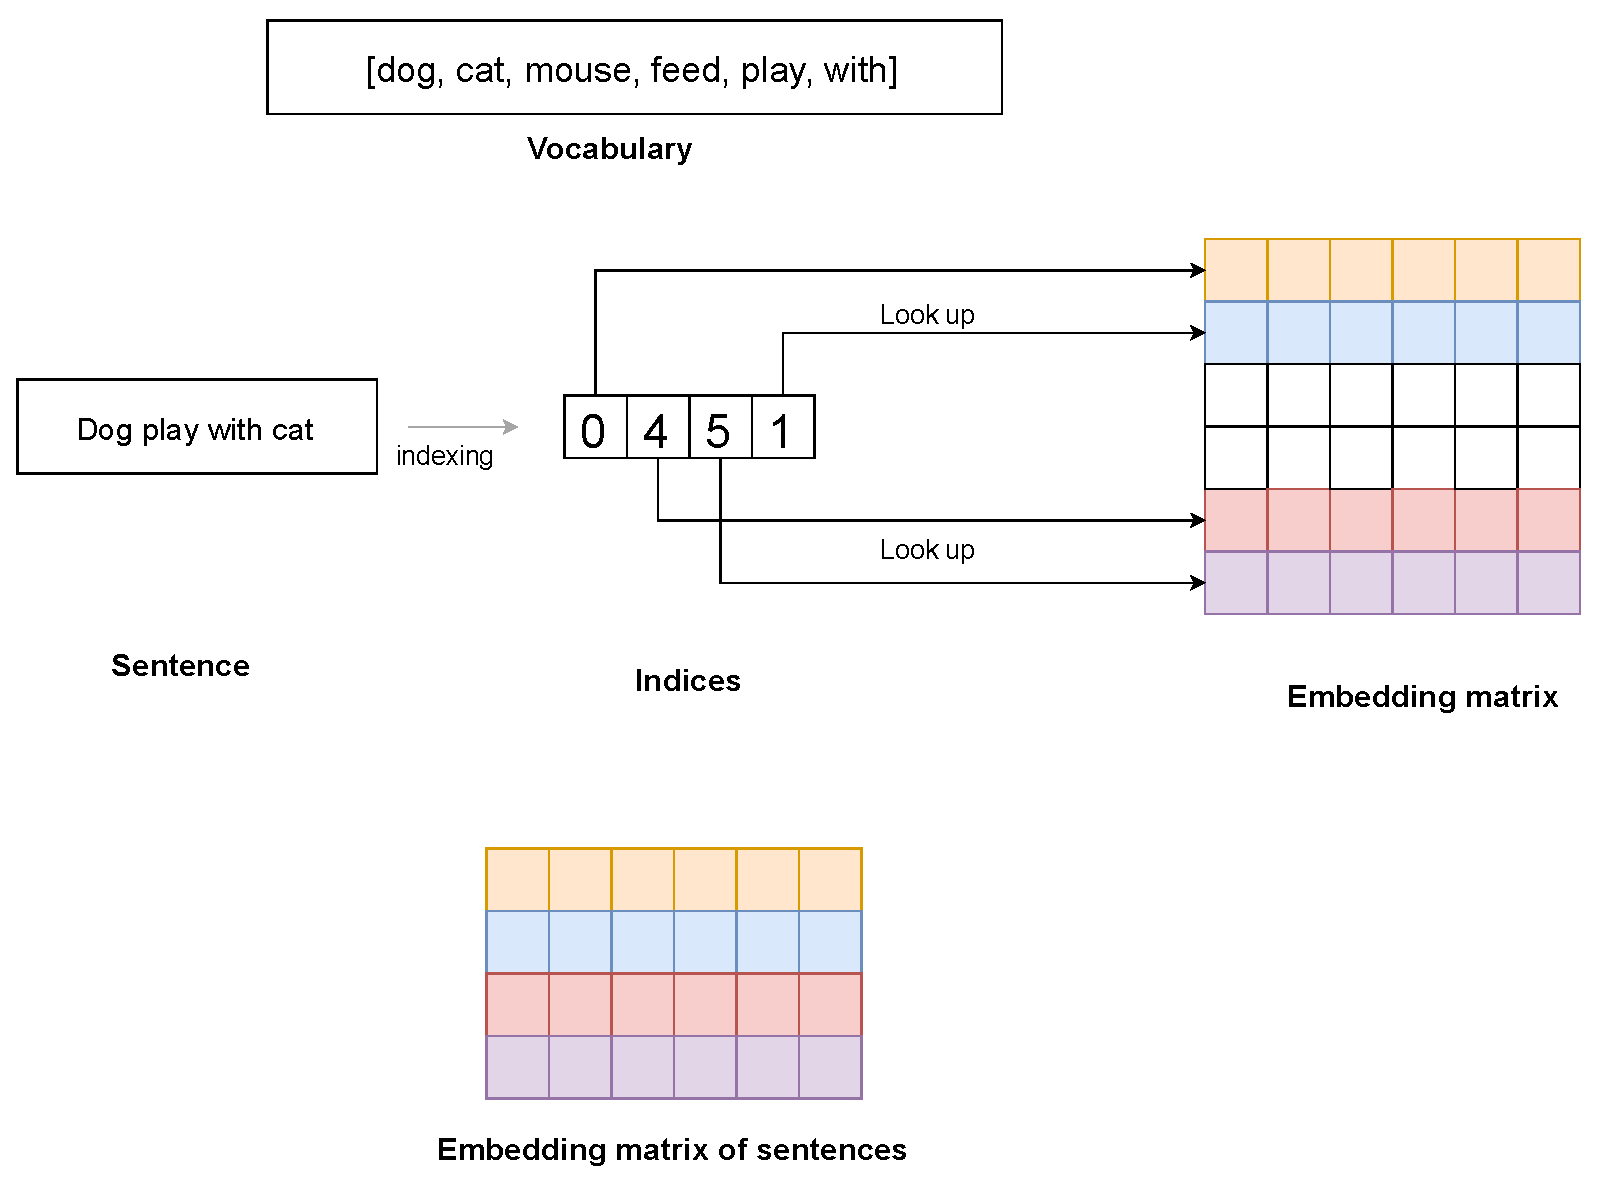
\includegraphics[width=0.9\linewidth]{figure/embeddinglayer.pdf}
	\caption[Overview of embedding layer]{Overview of Embedding Layer}
	\label{fig:embeddinglayer}
\end{figure}
\paragraph{Matrix presentation of sequences of words}
Given any sentence \(s\) of length \(n\), we denote \(x_i \in \mathbb{R}^d\) as a vector presentation of word-\(i\)th in the sentence.
Note that the first word in a sentence is word-\(0\)th, if the sentence is padded with dummy words on its left, these padded dummy words are indexed by negative integers.
Any sequence of words in the sentence which start at word-\(i\)th and end at word-\(j\)th can be presented as the following:
\begin{align}
X_{i:j} &= x_i \oplus x_{i+1} \oplus ... \oplus x_{j} &\label{concat}
\end{align}
In Eq.\eqref{concat}, \(\oplus\) is concatenation operator which result in the matrix \(X_{i:j} \in \mathbb{R}^{d \times (j-i+1)}\).


\subsection{Convolution Layer}
Given that \(F\) is the set of all filters of the convolution layer, for any filter \(v \in F\) which has window size \(l\) and set of parameters \(\theta^{(v)} = \{ W^{(v)}, b^{(v)} | W^{(v)} \in \mathbb{R}^{d \times l}, b^{(v)} \in \mathbb{R}\}\), filter \({v}\) is applied on any sequence of word-\(i\)th to word-\((i+l-1)\)th through the following equation:
\begin{align}
c^{(v)}_j &= f(W^{(v)} \otimes X_{i:i+l-1} + b^{(v)}) &\label{filter}
\end{align}

In Eq.\eqref{filter}, operator \(\otimes\) is the Hadamard product~\cite{element-prod}.  
\(b \in \mathbb{R}\) as bias term and \(f\) is an activation function.
For indexing, \(j = i + x\) with \(x \in \mathbb{N}\) and \(0 \leq x < l\).
If half-padding policy is employed then \(j = i + \floor{\frac{l}{2}}\).
For the case of multichannel input, given that the sentence is presented by any set of input channels \(Z\).
We will modify Eq.\eqref{filter} as follow:
\begin{align}
\forall h \in Z, \; \; \hat{c}^{(v)}_{jh} &= f(W^{(v)} \otimes X_{i:i+l-1} + b^{(v)})& \\
c^{(v)}_j &= \sum_{h \in Z} \hat{c}^{(v)}_{jh}&
\end{align}

By slicing the filter \(v\) through the sentence (i.e. applying the filter \(v\) on different sequences of length \(l\) along the sentence) we can get vector \(c^{(v)} = [c^{(v)}_0, c^{(v)}_1~\cdots]\) which is a feature map of the sentence \(s\).

\begin{figure}[H]
	\centering
	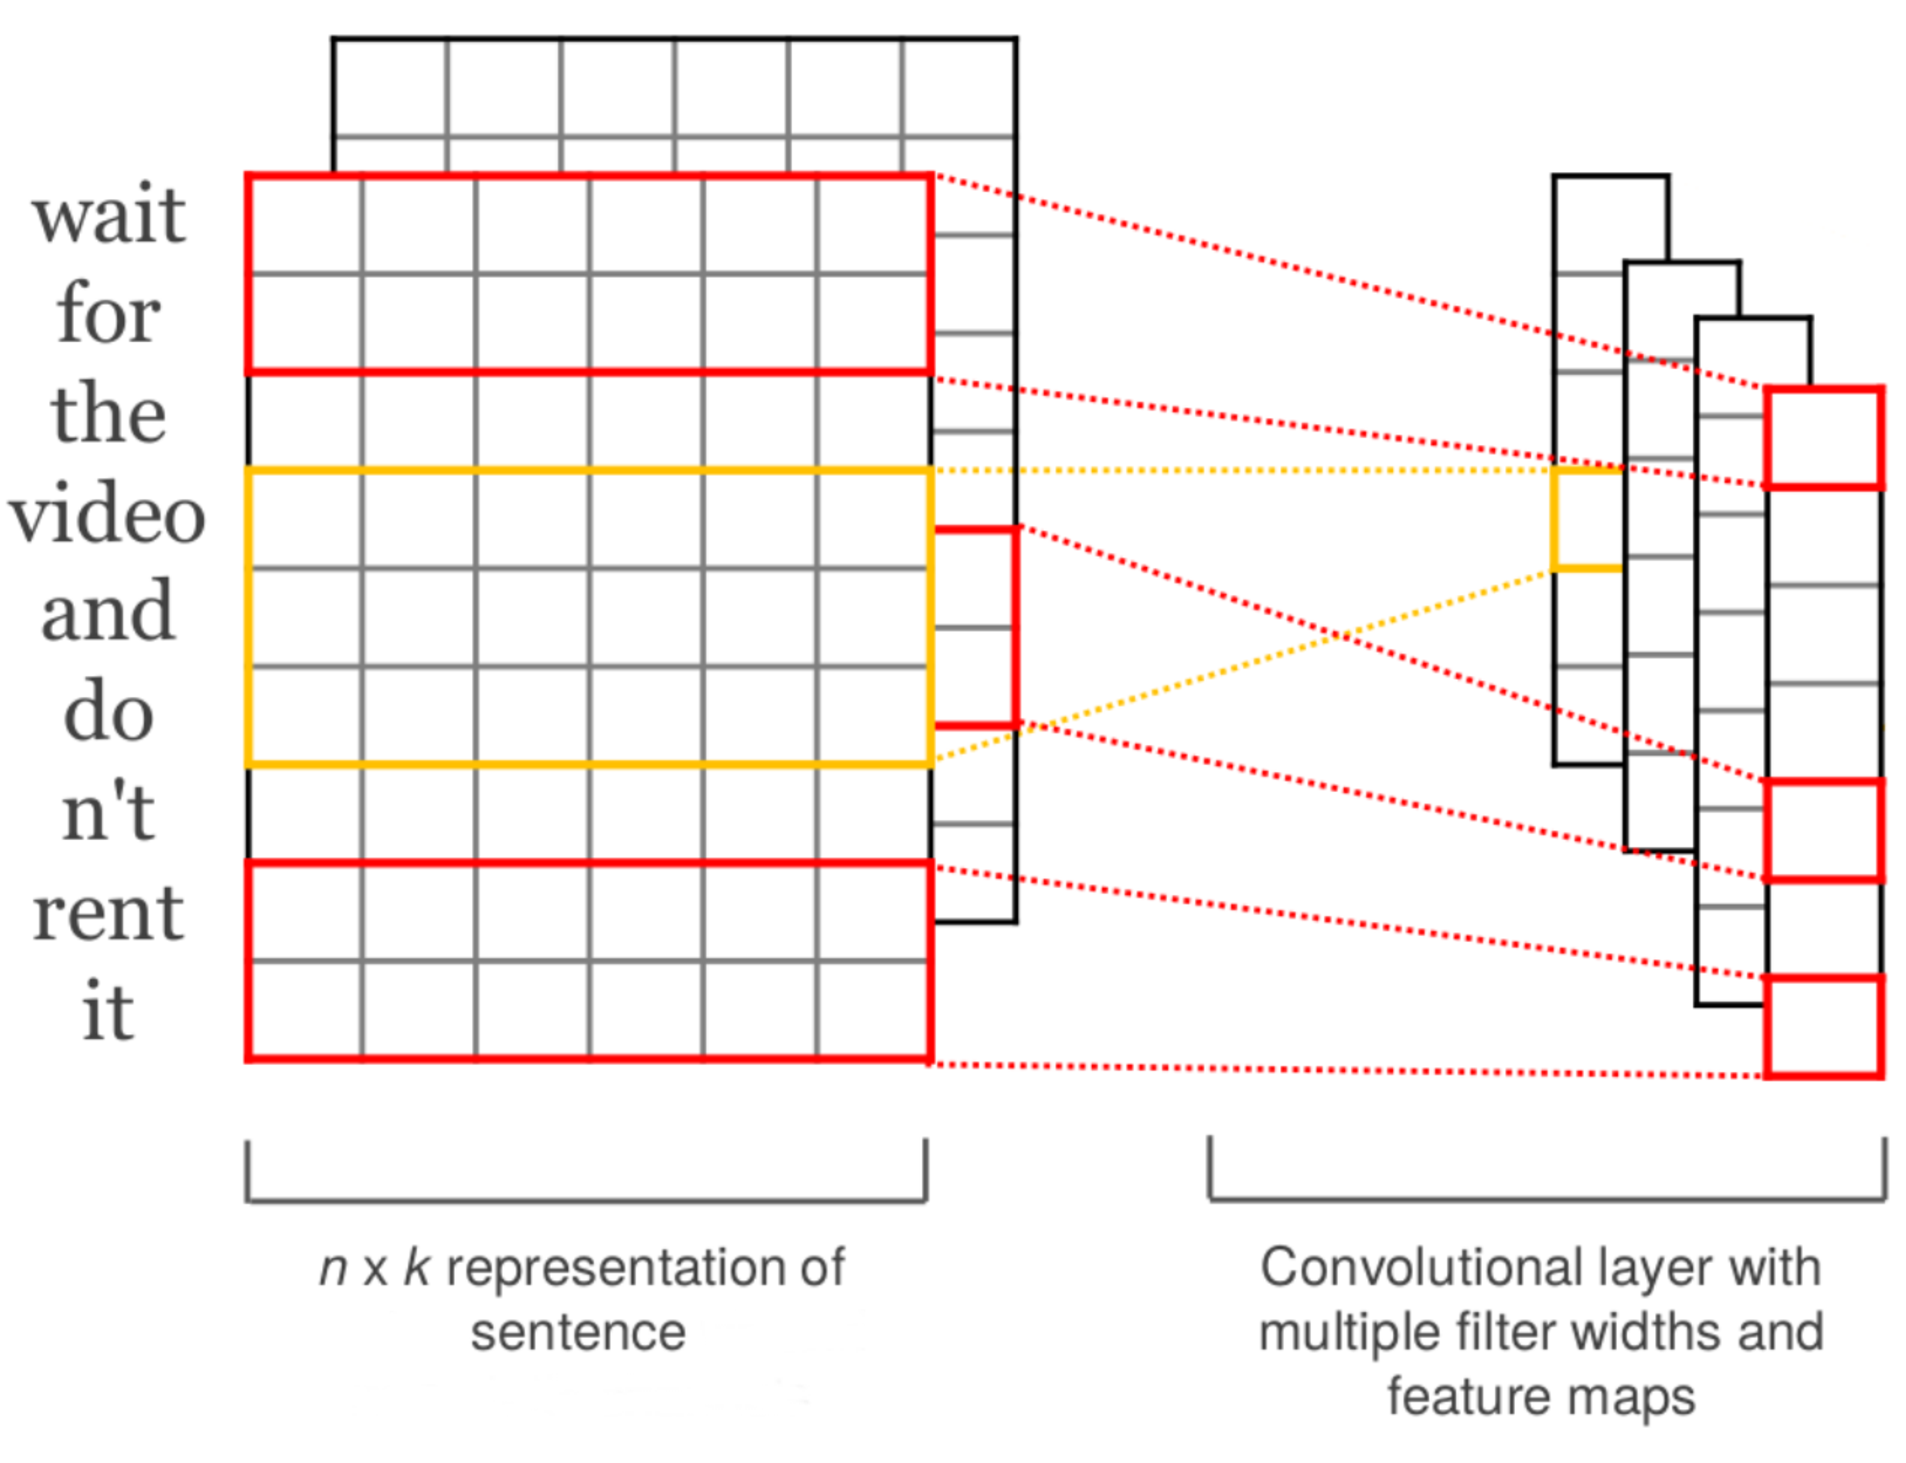
\includegraphics[scale=0.25]{figure/cnn-module}
	\caption[Convolution layer with two input channels]{Convolution layer with two input channels}
	\label{fig:cnn-module}
\end{figure}

Until now, we have not define the length of the feature map \(c^{(v)}\). 
To be able to work with Tree-LSTM (which required tree-structured inputs), all the feature maps produced by the convolution layer need to have length equal to that of the sentence \(s\) (which is \(n\) in this case).
For satisfying this constraint, all filters in \(F\) are restricted to have odd window sizes and being applied on the sentence according to half padding, unit strides policy~\cite{conv-arith}.
These conditions entail \({\forall u \in F,  c^{(u)} \in \mathbb{R}^n}\)~\cite{conv-arith}.
We demonstrate this policy in Fig.\ref{fig:half-padding}.

\begin{figure}[H]
	\centering
	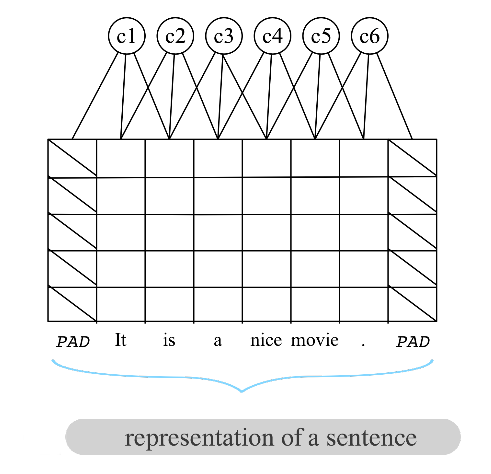
\includegraphics[scale=0.4]{figure/half-padding}
	\caption[Half padding, unit strides policy]{A convolution filter with window size 3 applying on a sentence according to half padding, unit strides policy.
		The length of the resulted feature map is equal to that of the sentence.}
	\label{fig:half-padding}
\end{figure}

Suppose the size of set of filters \(F\) is \(m\), all the feature maps produced by the set of filters is then concatenated into one matrix \(P \in \mathbb{R}^{m \times n}\), which each of its row is a feature maps.
After that, the column vectors of \(P\) are treated as input vectors for Tree-LSTM or any Recurrent Neural Network.
\subsection{Recursive Neural Network}
For this module, we reused Constituency Tree-LSTM~\cite{treeLSTM}.
Let \(d\) be the size of the input vectors, \(r
\) be the size of the memory cell and \(z\) be the number of sentiment classes. 

\paragraph{Leaf module}
Given any input vector \(x \in \mathbb{R}^d\), the calculation steps inside the leaf module can be expressed as follow:
\begin{align}
o &= \sigma{\left( W^{(o)} x + a^{\left(o\right)}\right)} & \\
c &= W^{(c)} x + a^{(c)} & \\
h &= o \odot \tanh{\left(c\right)} &
\end{align}

In this module, \(W^{(o)}, W^{(c)} \in \mathbb{R}^{r \times d}\) and \(a^{\left(o\right)}, a^{(c)} \in \mathbb{R}^r\).

\paragraph{Composer module}
Given the input vectors \({h_l}\), \({c_l}\) from the left child node and \({h_r}\), \({c_r}\) from the right child node, the calculation steps inside the composer module can be expressed as follow:
\begin{align}
i &= \sigma{ \left(U_l^{(i)} h_{l} + U_r^{(i)} h_{r} + b^{(i)} \right) } &\\
f_{l} &= \sigma{\left(U_{l}^{(l)} h_{l} + U_{r}^{(l)} h_{r} + b^{(f)}\right)} & \\
f_{r} &= \sigma{\left(U_{l}^{(r)} h_{l} + U_{r}^{(r)} h_{r} + b^{(f)}\right)} & \\
o &= \sigma{\left( U_l^{(o)} h_{l} + U_r^{(o)} h_{r} + b^{(o)}\right)} &\\
u &= \tanh{\left( U_l^{(u)} h_{l} + U_r^{(u)} h_{r} + b^{(u)}\right)} &\\
c &= i \odot u + f_{l} \odot c_{l} + f_{r} \odot c_{r} & \\
h &= o \odot \tanh{\left(c\right)} &
\end{align}

In this module, for any \(j \in \{i, l, r, o, u\}\) and \(x \in \{\l, r\}\), \(U_x^{(j)} \in \mathbb{R}^{r \times r}\) and \( b^{(j)} \in \mathbb{R}^r\).

\paragraph{Composing sentence}
Given any sentence \({s}\) of length \({n}\) and its parse tree, originally, Tree-LSTM composes the output vectors by first applying its leaf module on each word vectors then applying its composition function at each node of the parse tree in a bottom-up manner.
The output module is applied at the output \({h}\) of each node which has a sentiment label.

In case convolution layer was added, the only different is that for all \(0 \leq i \leq n-1\), the vector presentation of the word-\({i}\)th is replaced with the \({i}\)th-column of the matrix \({P}\) produced by the convolution layer.
This mean the size of input vectors \(d\) is equal to the number of filters \(m\).

\subsection{Output Module and Loss Function}
 Denoting sequence of words spanned by a sub-tree rooted at node \({j}\) as \({\{x\}_j}\).
Given \({h_j}\) is the \({h}\) ouput of node \({j}\), the prediction at node \({j}\) can be computed by the output module as follow:
\begin{align}
\hat{p_{\theta}}(y \mid \{x\}_j ) &= softmax( W^{(s)} h_j + b^{(s)}) & \\
\hat{y_j} &= \underset{y}{\mathrm{argmax}} \; \hat{p_{\theta}}(y \mid \{x\}_j ) &
\end{align}

In this module, for any \(W^{(s)} \in \mathbb{R}^{z \times r}\) and \( b^{(s)} \in \mathbb{R}^z\).
For loss function, negative log-likelihood with \(L2\) regularization was used.
\section{Model Enhancements}
\subsection{Training Glove Vectors on Large Sentiment Dataset}
\subsection{Multichannel Input}
This method was introduced by Yoon Kim~\cite{KimCNN}.
Although in his paper, in the training process of his 2-channel-CNN, Kim updated one channel and kept the other unchanged, we are not restricted ourselves to this rule.
The type of word embeddings used in each channel, the number of channels and the method for updating each channel are treated as hyper-parameters.

This method allows multiple parallel embedding layers in our model.
In other words, each word is presented by multiple vector representations.

\section{Experiments}
\subsection{Datasets}
\subsubsection{Stanford Sentiment Treebank} \label{sec:sst}
In this thesis, we used Standford Sentiment Treebank (SST) dataset~\cite{socher2013recursive} to evaluate our models sentence-level sentiment analysis task.
Originally, the dataset was built based on Rotten Tomatoes Movie Review dataset~\cite{Rotten-Tomato}~\cite{socher2013recursive}.
In total, Standford Sentiment Treebank contains 11,855 sentences.
The dataset was split into training, validation and test set which contains 8544, 1101 and 2210 sentences respectively.


In this dataset, every sentence was parsed using Stanford (constituency) parser~\cite{socher2013recursive}\footnote{Open source tool: \url{https://stanfordnlp.github.io/CoreNLP/}}, each phrase which is spanned by any sub-tree of the parse tree is then labeled with  a fine-grained sentiment label (see \textbf{Figure \ref{fig:sst}}).
Fine-grained sentiment is a setting which partition all sentiments into 5 classes: "Positive", "Somewhat Positive", "Neutral", "Somewhat Negative" and "Negative"~\cite{socher2013recursive} (a.k.a. \textbf{Fine-grained setting}).
There are total 215,154 phrases in the whole dataset.

For \textbf{Binary setting}, there are only to sentiment classed on the entire dataset, which means all neutral sentiment sentences are removed, "Positive" and "Somewhat Positive" are merged into one class, the same rule applied on "Somewhat Negative" and "Negative"~\cite{socher2013recursive}.
After all "Neutral" sentences have been removed, there are 6920/872/1821 sentences remained in train/dev/test set.

For training a Recurrent Neural Network on this dataset, any phrase which is spanned by a labeled node is treated as a training example. 

\subsubsection{Amazon Reviews}\label{sec:amazon}
Amazon Reviews is a gigantic review dataset
which contains 142.8 million reviews from Amazon spanning May 1996 - July 2014\footnote{\url{http://jmcauley.ucsd.edu/data/amazon/}}.
Each review contains product review (rating, text, helpfulness vote) and metadata (descriptions, category information, price, brand, and image features)~\cite{amazon-reviews}.
In this thesis, we only used a small part of Amazon Reviews.
These parts include Amazon Movies and TV reviews (7,850,072 reviews)~\cite{mcauley2013hidden}, Amazon Book reviews (22,507,155 reviews) and the new Movies and TV reviews (4,607,047 reviews)~\cite{McAuleyTSH15}~\cite{HeM16}.

Listing \ref{lst:amzreview} is a sample of book reviews.
Amazon Book reviews and new Movies and TV dataset have the same format. Listing \ref{lst:oldamzreview} is a sample of Amazon Movies and TV reviews old dataset (7,850,072 reviews).

\begin{lstlisting}[caption={Amazon reviews sample},label={lst:amzreview}]
{
"reviewerID": "AH2L9G3DQHHAJ",
"asin": "0000000116",
"reviewerName": "chris",
"helpful": [5, 5],
"reviewText": "Interesting Grisham tale of a lawyer that takes millions of dollars from his firm after faking his own death. Grisham usually is able to hook his readers early and ,in this case, doesn't play his hand to soon. The usually reliable Frank Mueller makes this story even an even better bet on Audiobook.",
"overall": 4.0,
"summary": "Show me the money!",
"unixReviewTime": 1019865600,
"reviewTime": "04 27, 2002"
}
\end{lstlisting}

\begin{lstlisting}[caption={Old Amazon reviews sample},label={lst:oldamzreview}]
{
"reviewerID": "AH2L9G3DQHHAJ",
"asin": "0000000116",
"reviewerName": "chris",
"helpful": [5, 5],
"reviewText": "Interesting Grisham tale of a lawyer that takes millions of dollars from his firm after faking his own death. Grisham usually is able to hook his readers early and ,in this case, doesn't play his hand to soon. The usually reliable Frank Mueller makes this story even an even better bet on Audiobook.",
"overall": 4.0,
"summary": "Show me the money!",
"unixReviewTime": 1019865600,
"reviewTime": "04 27, 2002"
}
\end{lstlisting}

The differences between the old Amazon reviews dataset\footnote{\url{https://snap.stanford.edu/data/web-Amazon.html}} and new Amazon reviews dataset\footnote{\url{http://jmcauley.ucsd.edu/data/amazon/}} is that:
They were gathered using different crawling methods, the author also solved the duplication problem in new the dataset~\cite{amazon-reviews}.
Table \ref{table:moviereview} shows number of reviews by overall.

\begin{table}[H]
	\centering
	\caption{New Movies and TV dataset}
	\label{table:moviereview}
	\begin{tabular}{@{}lllc@{}}
		\toprule
		& \multicolumn{3}{l}{Number of reviews}                         \\ \midrule
		5-Star & 2761408 & \multirow{2}{*}{3618913} & \multirow{5}{*}{4607047} \\ \cmidrule(r){1-2}
		4-Star & 857505  &                          &                          \\ \cmidrule(r){1-3}
		3-Star & \multicolumn{2}{l}{415369}         &                          \\ \cmidrule(r){1-3}
		2-Star & 233221  & \multirow{2}{*}{572765}  &                          \\ \cmidrule(r){1-2}
		1-Star & 339544  &                          &                          \\ \bottomrule
	\end{tabular}
\end{table}

\subsection{Experiment Setups}
\subsubsection{Hyper-parameters and training}
For the models with only single input channel, we initialized word representation with Glove vectors~\cite{glove}.
With two word embeddings channels, we initialized one channel using Glove Common Crawl\footnote{\label{glovecommoncrawl}Common Crawl (840B tokens, 2.2M vocabularies, cased, 300d vectors, 2.03 GB download) publicly available at \url{https://nlp.stanford.edu/projects/glove/}} and the other using our Glove Amazon.

We tried a variety of convolution filters combination.
For single kernel size, we performed grid search on $\{100, 200, 300\}$ number of kernels of size $\{3, 5\}$.
For two different kernel size, we tried with $\{100, 200\}$ number of kernels for each kernel size.
Output matrices of different kernel sizes were concatenated as if they were with same kernel size.

Our model was trained using AdaGrad~\cite{duchi2011adaptive} with learning rate of $\{0.1,~ 0.05,~ 0.01\}$, L2 regularization of $\{1e^{-3},~ 1e^{-4}, ~ 1e^{-5} \}$, batch size of 25.
We manually update our word representation with learning rate $\alpha$ of $\{0.1,~0.05, ~0.01\}$ following Eq.\ref{eq:manuallyupdate}.
We regularized convolution layer with input dropout rate of 0.5 and output dropout rate of 0.2 in addition to dropout of rate 0.5 at output layer.
We applied the same hyper-parameters grid search for two channels convolution.
\begin{equation}
\label{eq:manuallyupdate}
w = w - \alpha\delta J(\theta)
\end{equation}

We found that 100 filters of size 3 words and 100 filters of size 5 words yield better results compared to single filters size or the number of filters larger than 200. We trained with Adagrad of learning rate of 0.01 and word vectors (updated manually) at learning rate 0.1 give the best result. We trained for 60 epochs for CNN Tree-LSTM and 20 epochs for CNN LSTM. Training 60 epochs on CNN LSTM did not yielded observable better result than 20 epochs.
\subsubsection{Glove Hyper-parameters and training}
We use Glove implementation\footnote{Publicly available on Github \url{https://github.com/stanfordnlp/GloVe}} to train word representation.
We set $x_{max} = 100$, vector size to 300, windows size to 20 and the minimum number of word occurrences to be included in the vocabulary to 5.
The training process took the plain text file produced by the \hyperref[sec:preprocessamazonglove]{preprocessing steps} as its input.
In total, the size of the corpus is 4.7 billions tokens.
After the training process, the resulting word embeddings has vocabulary size of 1,734,244.
We named this word embeddings Glove Amazon.
Apart from using Glove Amazon to replace Glove Common Crawl for initializing word embedding layer of Tree-LSTM, the whole training process and hyper-parameters are kept unchanged.
\subsection{Results and Discussion}

\begin{table*}[]
	\centering
	\caption[Experiment result on SST]{Experiment results of models evaluated on Stanford Sentiment Treebank with binary setting.
		The models which have both data of mean(std) and max are models which have been evaluated by us.
		For these models, we report mean, standard deviation and max of 5 runs.
		If a model has data of only mean(std) or only max, the data was taken from its originated research paper.
		If the data of both mean(std) and max is missing, the model was not evaluated yet.
		\textit{(*): Result reported by the original paper.}}
	\label{table:experimentresult}
	\begin{tabular}{c|lll}
		\textbf{Block}    & \textbf{Model}  & \textbf{Mean(std)} & \textbf{Max}   \\
		\Xhline{3\arrayrulewidth}
		\Xhline{3\arrayrulewidth}
		
		\multirow{4}{*}{A} & CNN-non-static~\cite{KimCNN} & - & 87.20\Tstrut \\
		& CNN-multichannel~\cite{KimCNN} & - & 88.10 \\
		& DCNN~\cite{DCNN} & - & 86.80 \\
		& MVCNN~\cite{2-layer-cnn} & - & 89.40 \\
		\hline
		\multirow{5}{*}{B} & LSTM~\cite{originLSTM}    & 86.64 (0.27) & 86.93  \\
		& BiLSTM~\cite{GravesLSTM}  & 85.80 (0.69) & 86.43   \\
		& 2-layer LSTM~\cite{GravesLSTM} & 86.30 (0.60) & - \\
		& 2-layer Bidirectional LSTM~\cite{GravesLSTM} & 87.20 (1.00) & - \\
		& DMN~\cite{attention-gru} & - & 88.60 \\
		\hline
		\multirow{5}{*}{C} & RNTN~\cite{socher2013recursive}  & - & 85.40  \\
		& DRNN~\cite{IrsoyDRNN} & - & 86.60 \\
		& TE-RNTN~\cite{tag-embedding-rnn} & - & 87.70 \\
		& Dependency Tree-LSTM  ~\cite{treeLSTM}  & 85.70 (0.30)  & 85.80 \\
		& Constituency Tree-LSTM ~\cite{treeLSTM} & 88.00 (0.40)    &   88.19\\
		\hline
		\multirow{3}{*}{D} & GICF~\cite{group-instance} & - & 85.70 \\
		& Paragraph-Vec~\cite{ParagraphVec} & - & 87.80 \\
		& LSTM (PARAGRAM-SL999)~\cite{wieting2015towards} & 87.98 (0.46) & 88.50 (89.20)*
		\\
		\hline
		\multirow{2}{*}{E}  & CNN GRU ~\cite{cnn-rnn}                    & 89.13 (0.29)  &  89.61 (89.95)*    \\
		& CNN LSTM ~\cite{cnn-rnn}                    & 89.43 (0.28)  & 89.72 (89.56)*\Bstrut    \\
		\Xhline{3\arrayrulewidth}
		\Xhline{3\arrayrulewidth}
		\multirow{2}{*}{F} & Constituency TE Tree-GRU                 & 87.65 (0.34) & 88.25\Tstrut \\
		& Dependency TE Tree-GRU                   & 87.13 (0.70)  & 88.00\Bstrut \\
		\hline
		\hline
		\multirow{1}{*}{G} & Constituency Tree-LSTM ~\cite{treeLSTM} (Glove Amazon) & 88.85 (0.44) & 89.35\Tstrut\Bstrut \\
		\hline
		\hline
		\multirow{3}{*}{H} & CNN LSTM                                 & 89.10 (0.39)  & 89.40 \Tstrut  \\
		& 2 Channel CNN LSTM                        & 89.54    (0.22) & 89.79    \\
		& Multichannel CNN LSTM (pretrained) & - & - \\
		\hline
		\multirow{4}{*}{I} & CNN Tree-LSTM                            & 88.82 (0.13) & 88.92 \\
		& CNN Tree-LSTM (Glove Amazon)             & 88.96 (0.24) & 89.18 \\
		& 2 Channel CNN Tree-LSTM  &\textbf{89.69 (0.36)} & \textbf{90.12}    \\
		& Multichannel CNN Tree-LSTM (pretrained)        & - & -        \\
	\end{tabular}
\end{table*}


% \textit{(***): CNN and LSTM layer are initialize using pre-trained parameters from Section \ref{sec:CNNtree}}

Experiment results are summaries in Table \ref{table:experimentresult}.
Table \ref{table:experimentresult} is divided into two parts.
The first part is from Block A to E, which contains all baselines model.
The second part is from Block F to I, which contains all models which were proposed and evaluated by us.

\textbf{Descriptions of each Block in the first part}:
\begin{description}
	\item[Block A] contains Multilayer Convolution Neural Networks models.
	CNN-non-static and CNN-multichannel~\cite{KimCNN} are single layer CNN.
	DCNN~\cite{DCNN} and MVCNN~\cite{2-layer-cnn} are multilayer CNN, with MVCNN is a very large model  which has 2 layers, 5 word embeddings channels and unsupervised pre-train using the method of Sentence Encoding.
	\item[Block B] contains sequential/recurrent models.
	LSTM~\cite{originLSTM}, BiLSTM~\cite{GravesLSTM}, 2-layer LSTM~\cite{GravesLSTM} and 2-layer Bidirectional LSTM~\cite{GravesLSTM} have been described in Sec.\ref{sec:RNN}.
	DMN~\cite{attention-gru} is a sophisticated model used GRU with attention mechanism and episodic memory.
	\item[Block C] contains models which belong to the family of Recursive Neural Networks (tree-structured model).
	RNTN~\cite{socher2013recursive} is the first recursive neural network to successfully apply on sentence-level sentiment analysis (Stanford Sentiment Treebank).
	It was inspired by the idea that natural languages have recursive structure, to understand a sentence we must understand its phrases and, to understand a phrase, we must understand its words.
	DRNN~\cite{IrsoyDRNN} is a multilayered extension of RNTN.
	TE-RNTN is also an extension of RNTN which utilize the local syntactic information at each node of a sentence's parse tree.
	Dependency and Constituency Tree-LSTM~\cite{treeLSTM} are tree-structured versions of LSTM which have been described in Sec.\ref{sec:treelstm}.
	
	\item[Block D] contains transfer learning methods, which utilized a large amount of data other than Stanford Sentiment Treebank.
	GICF~\cite{group-instance} is an attempt to learn to classify sentiments of sentences (in Stanford Sentiment Treebank) from training dataset which contains only document-level sentiment labels.
	Paragraph-Vec~\cite{ParagraphVec} is a method that learns to encode any sequence of words into a vector with the purpose of maximizing the likelihood of words which appear in that sequence given the encoding vector.
	LSTM (PARAGRAM-SL999)~\cite{wieting2015towards} is a LSTM models with word embeddings layer initialized by PARAGRAM-SL999, word vectors trained on a large paraphrase dataset (PPDB~\cite{ganitkevitch2013ppdb}) % which was trained using a large paraphrase dataset (PPDB~\cite{ganitkevitch2013ppdb}).
	In our experiments with LSTM (PARAGRAM-SL999), we used the implementation and pre-trained word vectors which are publicly available on the author website\footnote{\url{http://ttic.uchicago.edu/~wieting/}}.
	
	\item[Block E] contains models which combine Convolution Neural Networks and Recurrent Neural Networks.
	CNN GRU and CNN LSTM~\cite{cnn-rnn} have been described in detail in Sec.\ref{cnn-rnn}.
	In our experiments with CNN GRU and CNN LSTM, we used the implementation publicly published by the authors\footnote{\url{https://github.com/ultimate010/crnn}}.
\end{description}
\subsubsection{Transfer Learning by retraining Glove on Amazon Reviews dataset}
\label{fact:glove-amazon-improve-tree}
In Block G, Constituency Tree-LSTM using Glove Amazon largely outperformed Constituency Tree-LSTM using Glove Common Crawl even though it was trained on significantly larger dataset (840B tokens) compared to our preprocessed Amazon Reviews (4.7B tokens) (Sec.\ref{sec:gloveamazone}).
This method also outperformed all the Transfer Learning methods in Block D.
Compared to Glove Amazon method, originally,  Paragraph-Vec~\cite{ParagraphVec} cannot be fine-tuning in a supervised manner.
We also used PARAGRAM-SL999 for initializing the word embeddings layer of Constituency Tree-LSTM,
the results (of 8 runs with mean 87.175\% and standard deviation 0.69) were not as good as those of Glove Common Crawl.

These results support our hypothesis that by training word embeddings on review documents, especially movie or book reviews, we can capture more rare words and also the different way people use words (or different word relationships) when they express their opinions on movies or books (Sec.\ref{movie-hypothesis}).

\subsubsection{Combining Recursive Neural Networks with Convolution Neural Networks}
\label{proved:tree-conv-benefit}
The fact that CNN Tree-LSTM outperforms Constituency Tree-LSTM~\cite{treeLSTM} supports our hypothesis on the benefits of combining convolution layers with Tree-LSTM (Sec.\ref{conv-tree-benefits}).
Due to using similar architects, CNN LSTM was comparable with CNN GRU and CNN LSTM~\cite{cnn-rnn}. \label{unproved:cnn-treelstm-overfit}
CNN Tree-LSTM performed worst than CNN LSTM, the reason might because of over-fitting.
We will prove this hypothesis by looking at the plots of error rate on training and validation set of these two models.

\label{proved:Amazon-adv-Common}
We have seen that Glove Amazon improved Tree-LSTM in Sec.\ref{fact:glove-amazon-improve-tree}.
In these experiments (Block I), Glove Amazon also improved CNN Tree-LSTM.
We can conclude that Amazon Glove captured some good\footnote{good for the task of sentiment analysis of movie reviews} features that does not exist or hardly be extracted in Glove Common Crawl.

According to Table.\ref{table:paramtable}, the number of parameters of 2 Channel CNN Tree-LSTM (722,153) is much larger than that of CNN Tree-LSTM (482,153), which makes it more likely for 2 Channel CNN Tree-LSTM to over-fit the training data.
However, in fact, 2 Channel CNN Tree-LSTM was able to archive much higher accuracy than both CNN Tree-LSTM (Glove Amazon) and CNN Tree-LSTM (Glove Common Crawl).\label{proved:Common-syn-Amazon}
The result proves that there are some features only appearing in Glove Common Crawl or when combining both Glove Amazon and Glove Common Crawl.
Otherwise, there would not be any improvement.

\section{Conclusion}
\subsection{Contributions}
In search of new improvements on the task of sentence-level sentiment analysis, we have tried three approaches: Utilizing local syntactic information at each node of Recursive Neural Networks; Transfer Learning by retraining Glove on Amazon Reviews dataset and Combining Recursive Neural Networks with Convolution Neural Networks.
\textbf{Hypotheses that supported by our experiment results including}:
\begin{itemize}
	
	\item For sentence-level sentiment analysis on movie reviews, there exist useful features in Glove Amazon which does not exist or hardly be extracted in Glove Common Crawl.
	On the other hand, there also exist useful features that does not appear in Glove Amazon but only appear in Glove Common Crawl or when combining both Glove Amazon and Glove Common Crawl.
	
	\item By adding a convolution layer before the leaf-module of Tree-LSTM, the convolution layer will help Tree-LSTM to mitigate the problem of lacking local context and weak feature capturing at leaf nodes.
	Mutually, using Tree-LSTM to combine the feature maps produced by convolution layer is better than max-over-time pooling layer.
	
	\item  Tree-LSTMs have already utilized the information in word embeddings and the local syntactic information from tag embeddings adding no more value. 
\end{itemize}

\subsection{Future works}
\label{unproved-hypo}
\textbf{Hypotheses that we have not had efficient data to support or oppose}:

\begin{itemize}
	\item Unsupervised pre-training methods (on Amazon Reviews) can help improving Multichannel CNN LSTM and Multichannel CNN Tree-LSTM. (Sec.\ref{sec:unsupervised-pretrain})
	
	\item In many cases, words or phrases have different meaning depend on their contexts.
	By pre-training Multichannel CNN LSTM as Language Model, these information about how to compose words can be embedded in word embeddings or parameters of the model.
	
	\item By training as Language Model on part of Amazon Reviews dataset, Multichannel CNN LSTM can learn more specific dependencies: The reviewer cries when watching a good romantic movie, or the viewer praises the novel and then criticizes the movie based on how good the novel is, or how sentiments being affected by sentence structures. 
	
	\item CNN Tree-LSTM performed worst than CNN LSTM, the reason might be because of over-fitting. (Sec.\ref{unproved:cnn-treelstm-overfit})
\end{itemize}

We will do experiments to have efficient data to support or oppose the unproved hypotheses above.
We will also re-evaluate our models and methods on Stanford Sentiment Treebank with fine-grained setting.

In many cases, the sentiment class of a sentence can only be revealed through multiple steps of induction and deduction on a knowledge base.
We suspected that most of the networks we have done experiments with (e.g. Tree-LSTMs, CNN-multichannel and our model) do the sentiment classification task based on detecting features and do not rely on induction or deduction.
We thinks that most of the knowledge these models have is embedded in their word embeddings (which have 6,255,600 parameters or double that number in case of two input channels compared to 722,153 parameters at most in these neural networks).

In recent years, Recurrent Neural Networks with external memory~\cite{Graves_Nature2016}~\cite{neural-turing-machine} have come into sight.
DNC~\cite{Graves_Nature2016} was proved to have certain level of reasoning on the bAbI dataset~\cite{bAbi}.
We hope that we can apply this reasoning ability on sentence-level sentiment analysis.

\appendix
%Appendix A

\begin{acks}
  The authors would like to thank Dr. Yuhua Li for providing the
  matlab code of  the \textit{BEPS} method. 

  The authors would also like to thank the anonymous referees for
  their valuable comments and helpful suggestions. The work is
  supported by the \grantsponsor{GS501100001809}{National Natural
    Science Foundation of
    China}{http://dx.doi.org/10.13039/501100001809} under Grant
  No.:~\grantnum{GS501100001809}{61273304}
  and~\grantnum[http://www.nnsf.cn/youngscientsts]{GS501100001809}{Young
    Scientsts' Support Program}.

\end{acks}
